\documentclass[12pt,a4paper]{article}
\usepackage[utf8]{inputenc}
\usepackage{polski}
\usepackage{graphicx}
\usepackage{verbatim}
\title{Równoległe rozwiązanie problemu komiwojażera. Algorytm kolonii mrówek}
\author{Marcin Fabrykowski, Jan Kleszczyński}
\begin{document}
\maketitle
\newpage
\section{Opis problemu}
Problem komiwojażera jest podstawowym zagadnieniem logistycznym. Polega on na znalezieniu
najtańszej drogi między miastami, w sposób, który pozwala odwiedzić każde miasto tylko jeden raz.
Zauważono, że mrówki, które wyruszają z mrowiska na poszukiwanie pożywienia, po znalezieniu jego źródła zaczynają poruszać się najkrótszą możliwą ścieżką. Dalsze obserwacje zdradzają nam
następujący algorytm:
\begin{enumerate}
\item Każda mrówka wyrusza na poszukiwania i obchodzi raz każde ze źródeł pożywienia, po czym
wraca do mrowiska.
\item Przechodząc po ścieżce, jeżeli jest ona krótsza od poprzedniej, pozostawia feromony.
\item Feromony każdej z mrówek sumują się, lecz co pewien czas parują.
\item Przy następnym wyjściu z mrowiska, mrówka decydując o wyborze drogi pokieruje się do
miasta, do którego droga zawiera najwięcej feromonów. Jednakże każda mrówka ma swoją
ciekawość, która również zostanie uwzględniona.
\item Po pewnym czasie mrówki zaczną wybierać zawsze tą samą trasę, która jest trasą najkrótszą.
\end{enumerate}
W celu zrównoleglenia tego problemu zastosowaliśmy algorytm widoczny poniżej na schemacie.
Mrówek jest tyle ile miast i są równomiernie rozłożone pomiędzy procesy. Gdy liczba miast jest nie podzielna przez ilość procesów reszta z dzielenia jest dodawana do procesu o ranku równym 0. 
\section{Opis algorytmu}
Algorytm zastosowany w programie przedstawia się w następujący sposób:
\begin{enumerate}
\item Wczytanie mapy.
\item Przekazanie jej do wszystkich hostów. (pierwsze zrównoleglenie)
\item Określenie ilości mrówek.
\item Wyruszenie przez mrówki na wędrówkę
\begin{itemize}
\item Wybór ścieżki (powtarzany aż do przejścia przez każde miasto)
\end{itemize}
\item W tym miejscu wszystkie mrówki przeszły przez wszystkie miasta i znane są ich trasy oraz długości drogi.
\item Parowanie feromonów
\item Określenie która ze ścieżek jest najkrótsza na danym hoście.
\item Przesłanie długości najlepszej ścieżki (pierwsza redukcja)
\item Wybór najlepszej ścieżki z nadesłanych.
\item Rozesłanie informacji o identyfikatorze hosta z najlepszą ścieżką (drugie zrównoleglenie).
\item Sprawdzenie, czy identyfikator hosta zgadza się z identyfikatorem rozesłanym przez proces zarządzający. Jeżeli nie to skok do punktu 13.
\item Rozesłanie najlepszej ścieżki do wszystkich hostów.
\item Rozłożenie feromonów na otrzymanej ścieżce (najlepszej ze wszystkich innych).
\item Przesłanie decyzji o zakończeniu (druga redukcja).
\item Jeżeli wszystkie mrówki przeszły nie więcej niż dwoma trasami i wykonano co najmniej 50 iteracji, aplikacja kończy działanie, drukuje długość znalezionej trasy i zapisuje szczegółowe informacje o trasie do pliku. W przeciwnym razie następuje skok do punktu 3.
\end{enumerate}
Schemat blokowy przedstawiony jest na Rys. \ref{fig:schemat}
\begin{figure}
\vspace{-4.5cm}
\caption{Schemat blokowy algorytmu}
\label{fig:schemat}
\hspace{-2cm}
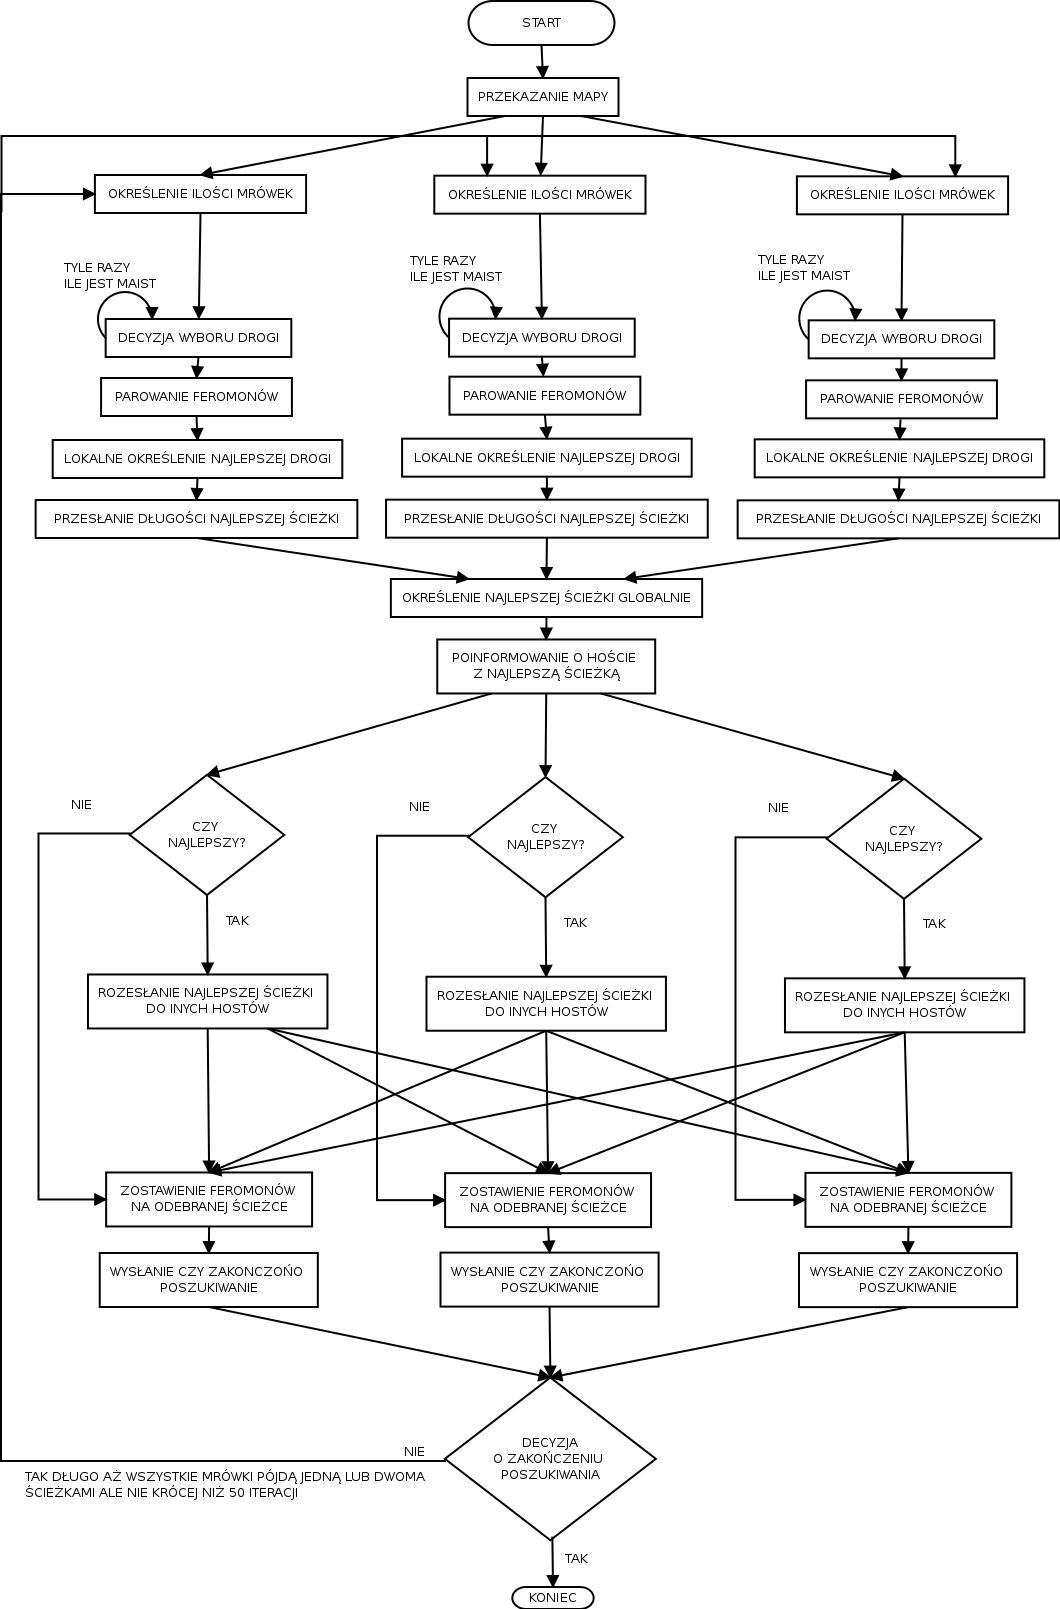
\includegraphics[scale=0.5]{schemat.png}
\end{figure}
\section{Informacje o danych we/wyjściowych}
Plik map.ini zabierający następujące dane:\\
$c <liczba:num>$ -- liczba miast\\
$r <src:num>\ <dst:num>\ <len:num>$ -- definicja drogi\\
$\#$ -- komentarz\\
W wynikowym pliku wynik.txt znajduje się długość trasy oraz kolejność przechodzenia przez miasta. 
\section{Uruchomienie}
W celu uruchomienia aplikacji należy wykonać następujące komendy:
\begin{verbatim}
./configure
make
make run
\end{verbatim}
Spowoduje to sprawdzeniem systemu pod kątem zgodności, skompilowaniem aplikacji oraz jej uruchomieniem.
\end{document}
